\documentclass[a4paper,french,oneside,twocolumn,10pt,]{memoir}

% TITLEPAGE
\newcommand*{\myunilogo}{Figures/logos/GitHub_Lockup_Black.png}      % insert file path
\newcommand*{\mylablogo}{Figures/logos/GitHub_Lockup_Black.png}      % insert file path
\newcommand*{\myhostunilogo}{Figures/logos/GitHub_Lockup_Black.png}  % insert file path

\renewcommand*{\author}{mlagg}
\newcommand*{\myemail}{tung@gmail.com}

\title{Ici mettre l'intitulé du rapport}
\newcommand*{\documenttype}{Un rapport qui rapporte}

\newcommand*{\tutor}{Tung Tung Sahur}
\newcommand*{\tutoremail}{tung@gmail.com}

\newcommand*{\PI}{Gaëtan Le Singe}
\newcommand*{\PIemail}{tung@gmail.com}

\newcommand*{\SchoolSupervisor}{Buffalo Drill}
\newcommand*{\SchoolSupervisoremail}{tung@gmail.com}

\newcommand*{\timespend}{Octobre 2026 $-$ Octobre 2050}

\newcommand*{\myhomeuni}{Université des hommes poires}
\newcommand*{\mymastersname}{Ingénieur en leadership}

\newcommand*{\myerasmusuni}{Université de Tenerife}
\newcommand*{\myerasmusmastersname}{Master poulet}

% Other PDF properties
\newcommand*{\keywords}{kw1,kw2,...}
\newcommand*{\subject}{research field}
			% pdf and titlepage infos
\usepackage[provide=*]{babel}
\usepackage{datetime2}
\DTMsetup{useregional}

\usepackage[table,dvipsnames]{xcolor}
\definecolor{ecnblue}{RGB}{16,28,72}
\definecolor{ecnyellow}{RGB}{250,182,0}
\colorlet{titlecolor}{ecnblue}
\colorlet{secondarycolor}{ecnyellow}
\definecolor{insared}{RGB}{238,28,34}
\definecolor{insagrey}{RGB}{79,77,80}

% For tikz and pgf plots
\usepackage{tikz}
\usetikzlibrary{calc}
\usepackage{tikz-cd}
\usepackage{progressbar}
\usetikzlibrary{shapes.geometric}
\usetikzlibrary{babel}
\usepackage{pgfplots}
\usepackage{import}
\pgfplotsset{compat=1.14}
\def\mathdefault#1{#1} 			% avoid pgf bug from plt figure export
\usepackage{xsavebox} 			% save content for repeated use
\usepackage{atbegshi} 			% insert material on every page
\usepackage[texcoord=true]{eso-pic} % The zero point of the coordinate system is the upper left corner of the page.

% Maths set up 
\usepackage[retainorgcmds]{IEEEtrantools} % utlime equation envir. (see guide in LateX folder on Chrome)
\usepackage[intlimits,  	% places super/subscript on top of the integral sign
			reqno,      	% Place equation numbers on the right.
			]{amsmath} 
\usepackage{amsfonts}
\usepackage{amssymb}		% nice math symbols
%\usepackage{esvect} 		% vector sign tuning : \vv{e}{1} does not put arrow over subscript \vv{e_1} does
\usepackage{exscale} 		% to get the sum sign right (bigger)
\usepackage{xfrac} 			% nice inline fraction with \sfrac command

% Physics and chemistry 
\usepackage{siunitx}
\usepackage[version=4]{mhchem}
%\usepackage{chemfig}
%\usepackage{chemformula}

% Code
\usepackage{piton}           % shows code nicely
\usepackage{tcolorbox}       % box the pyhton code in a frey shaded box
\tcbuselibrary{breakable}    % idk

%\DeclareMathOperator{\logd}{$\mathrm{log}_2$} % example of the command \logd in math mode which write log_2 in upwrite nicely
\newcommand{\vect}[1]{\vec{#1}}  % example of a new command \vect for writing bold vectors
\newcommand{\overbar}[1]{\mkern1.5mu\overline{\mkern-1.5mu#1\mkern-1.5mu}\mkern 1.5mu}


% Bibliography 
\usepackage[sorting=none,      		% sorts by citation order
			citestyle=numeric-comp, % number style and concatenation
			autocite=superscript,
			language=french,
			style=nature,
			]{biblatex}
\usepackage{doi}

% Fonts

%lettrine stuff
\usepackage{lettrine,verbatim,longtable,url}
\usepackage{Konanur,Sanremo,Kramer,Typocaps}
\renewcommand{\LettrineFontHook}{\Typocapsfamily\color{insagrey}}
\renewcommand{\LettrineTextFont}{\color{insagrey}\scshape}

%first set up the main font
\usepackage{fontspec}
\setmainfont[Numbers = {OldStyle,Proportional},Ligatures=TeX,Microtype]{TeXGyrePagella}
\setsansfont[Microtype,Scale=MatchLowercase]{TeXGyreAdventor}
\newfontfamily\titlefamily{TeXGyreAdventor}[Microtype,Scale=MatchLowercase,LetterSpace=3]

\newfontfamily{\liningmainfont}[Numbers=Lining]{TeXGyrePagella}
\newfontface\heroscondensedbold{texgyreheroscn-bold.otf}[RawFeature = {+smcp}]
\newfontface\heroscondensedreg{texgyreheroscn-regular.otf}

%then set up the math font
\usepackage{unicode-math}
\setmathfont{TeX Gyre Pagella Math}

\linespread{1.05} 							% increase line spacing slightly
\usepackage[babel=true,nopatch=footnote]{microtype} 	% 'subliminal refinements towards typographical perfection'
\usepackage{romannum}

% Tables
\usepackage{tabularx} 		% automatically loaded with memoir, can fix the table width 
\usepackage{multirow} 		% ?
\usepackage{makecell} 		% retour à la ligne dans une cellule 
\usepackage{booktabs} 		% automatically loaded with memoir Required for better horizontal rules in tables

% Float captions
\usepackage{setspace}
\usepackage[font=small,
			textfont = {rm},
			format = plain,
			figureposition = below,
			tableposition = top,
			hypcap=true 			% for commands in caption (cite, math?)
			]{caption}
\DeclareCaptionFont{tc}{\color{titlecolor}}
\DeclareCaptionLabelSeparator{CapSep}{~\ding{71}~}
\captionsetup{labelfont={tc,sf,sc},labelsep=CapSep}

%Pages geometry
\usepackage[%showframe
]{geometry}
%\usepackage{pdflscape}
%\usepackage{rotating}
%\usepackage[export]{adjustbox}

\usepackage{csquotes}
\usepackage{textcomp} 				% for \textmu
\usepackage[language=french]{lipsum}
\usepackage{datatool-base}      	% for bib entries with ISBN
\usepackage{graphicx}
\usepackage{flafter}				% float appears after \ref. in text
\usepackage{pifont}					% for quick symbols, see https://lesfichesabebert.fr/TeX/latex/Listes.html
\usepackage[shortlabels]{enumitem}	% tuning listings environments
\usepackage{ragged2e}
\usepackage{todonotes}				% insert to do notes via \todo{}
\usepackage{titletoc}				% for \minitoc at chapter calls
\usepackage{cuted}					% for onecolumn domain w/o pageskips
\setlength{\stripsep}{0ex}
\usepackage{hyphenat}
\usepackage{etoolbox}
%\usepackage{lua-visual-debug}

\usepackage{hyperref}
\hypersetup{
	frenchlinks = true, 	% Use small caps instead of color for links.
	plainpages = false,
	colorlinks = true,
	linktocpage=true,		% numbers are only hyperlink in toc
	linkcolor = titlecolor,
	citecolor = titlecolor,
	urlcolor = titlecolor,
	pdfkeywords = \keywords,
	pdfsubject = \subject,
	pdfauthor = {\author},
	pdftitle = {\thetitle},
	pdfnewwindow = true, 	% new window for link to a place out of the doc
	pdfpagelayout = OneColumn,
	pdfstartview = FitBH,
	unicode = true, 		% permettre d’utiliser des caractères non-latins dans les marque-pages du lecteur de PDF
}

% Glossary
\usepackage[xindy={codepage=utf8}, 	% adding utf8 so that it works with Lua
	toc=true, 				% add glossaries to the toc.
	translate=babel, 		% If babel has been loaded, the translate=babel option is switched on
	%automake, 				% usable in unrestricted mode...
	%abbreviations,
	acronym, 				% add the category for acronyms
	symbols, 				% add the category for symbols
	%hyperfirst = false,	% idk
	%stylemods = mcols, 		% column style + correct style
	%style = mcolindex, 	% two column in textwidth
	%postdot, 				% puts a dot behind each entry
	nonumberlist, 			% no page refs in the glossaries
]{glossaries-extra}


%Usage:
%1.  add entry (e.g.\newabbreviation{svm}{SVM}{support vector machine}) in glossary.tex
%2. refers the glossary item in document by \gls{item}
%3. compile with cmd: >> makeglossary main 
%4. compile with cmd: >> lualatex main
%5. compile again: >> makeglossary main ,for news items refered in document

%\glsfmttext{label} using glossary entries in headings or labels


\addbibresource{myrefs.bib}
\makeglossaries 			% creates the xindy file main.xdy

% PAGE STEUP
\newcommand{\deadmarginlength}{3cm}
\newcommand{\bodytextlength}{17cm}
\newcommand{\pagewidthh}{21cm}

% from https://github.com/astoeckel/smart-thesis?tab=readme-ov-file
\settypeblocksize{23.45cm}{\bodytextlength}{*}
%\setlength{\textheight}{23.45cm}
%\setlength{\textwidth}{11.85cm}
\setlrmargins{2cm}{*}{*}
\setulmargins{*}{*}{*}\newcommand{\figlength}{\pagewidthh-2\deadmarginlength}

\setcolsepandrule{0.6cm}{0pt}						%space bewteen the 2 columns and thickness of the vertical rule in between
\checkandfixthelayout

% CONSTANTS
\newlength{\logopad}    	\setlength{\logopad}{14.279mm}
\newlength{\vertmargin}		\setlength{\vertmargin}{3.125cm}
\newlength{\xrule}			\setlength{\xrule}{-\vertmargin+\headsep}

%List
\setlist{noitemsep}
\setlist[1]{labelindent=\parindent}
\setlist[itemize]{leftmargin=0pt}
\setlist[itemize,1]{label=--}

% Abstract
\abstractcol 	% declaration specifies that an abstract in a twocolumn class option document should be typeset like a normal, unnumbered chapter. The
\abstractintoc 	% specifies that the abstract title should be added to the ToC. The declaration \abstractnum specifies that the abstract should be typeset like a numbered chapter

\renewcommand{\abstractnamefont}{\centering\large\scshape\sffamily\MakeLowercase} % same as section

% Bringhurst modified chapter style for front matter
\makechapterstyle{frontmatter}{%
	\renewcommand{\chapterheadstart}{}
	\renewcommand{\printchaptername}{}
	\renewcommand{\chapternamenum}{}
	\renewcommand{\printchapternum}{}
	\renewcommand{\afterchapternum}{}
	\renewcommand{\printchaptertitle}[1]{%
		\color{titlecolor}\sffamily\centering\large\scshape{##1}}
	\renewcommand{\afterchaptertitle}{%
		\vskip\onelineskip \vskip\onelineskip}
}

\newcommand{\ChapNumFont}{\color{titlecolor}\fontsize{30pt}{0pt}\titlefamily}
\newlength{\innersep}		\setlength{\innersep}{0.333em}
\newlength{\ChapNumWidth}
\newlength{\ChapNumheight}
\newlength{\cnh}
\newcommand{\halfboxsize}{0pt} % cmd to make it global

\makechapterstyle{main}{%
	\renewcommand*{\printchaptername}{}%
	\renewcommand*{\chapternamenum}{}%
	\renewcommand*{\chapnumfont}{\ChapNumFont}
	\renewcommand{\chapterheadstart}{}%
	\renewcommand*{\printchapternum}[1]{}
	\renewcommand*{\afterchapternum}{}%
	\renewcommand*{\printchapternonum}{}%
	\renewcommand*{\chaptitlefont}{\ChapNumFont\scshape}%
	\renewcommand*{\printchaptertitle}[1]{%
		\gdef\currentchaptertitle{##1}%
		\settoheight{\cnh}{\chaptitlefont ##1}%
		\settowidth{\ChapNumWidth}{\ChapNumFont \thechapter}%
		\settoheight{\ChapNumheight}{\ChapNumFont \thechapter}%
		\renewcommand{\halfboxsize}{\dimexpr\cnh/2+0.2cm+\innersep}%
		\begin{tikzpicture}[remember picture, overlay]
			\coordinate (origin) at ($(current page.north west)+(2cm,-3.125cm-\halfboxsize)$);%
			\def\boxlength{17cm-0.6cm-\ChapNumWidth-4\innersep}
			\filldraw[draw=titlecolor,fill = white] ($(origin)+(0,-\cnh/2-\innersep-0.2cm)$) rectangle ($(origin)+(17,\cnh/2+\innersep+0.2cm)$);%
			\node[fill = insagrey!10,text=titlecolor,anchor=west,text height = \cnh] at ($(origin)+(0.2cm,0)$) (A) {\chapnumfont\thechapter};%
			\node[fill = insagrey!10, right = 0.2cm of A,text width = \boxlength,text=titlecolor] (B) {\chaptitlefont ##1};%
			\node[fill=secondarycolor,right = 0pt of A ,text width=2pt-2\innersep,text height=\cnh-2\innersep,anchor=east] (C) {};
		\end{tikzpicture}%
	}%
	\renewcommand{\afterchaptertitle}{\vspace*{3\halfboxsize}}%
  }

% TOC STYLE
\newfontfamily\secfamily{TeXGyreAdventor}[Scale=MatchLowercase,]
\renewcommand{\cftchapterfont}{\secfamily\scshape}
\renewcommand{\cftchapterpagefont}{\secfamily}

\renewcommand{\cftsectionfont}{\color{titlecolor}\titlefamily\scshape}
\renewcommand{\cftsectionpagefont}{\color{titlecolor}\sffamily}

\renewcommand{\cftsubsectionfont}{\itshape\titlefamily}
\renewcommand{\cftsubsectionpagefont}{\sffamily}

\renewcommand{\cftfigurefont}{\sffamily}
\renewcommand{\cftfigurepagefont}{\sffamily}

\renewcommand{\cfttablefont}{\sffamily}
\renewcommand{\cfttablepagefont}{\sffamily}

% HEADER STYLES - Modified Bringhurst
%% Sections and subsections
\setsecnumformat{\liningmainfont\csname the#1\endcsname\quad}

%% The section style
\newcommand{\uppercasehead}[1]{%
	\noindent\tikz{\node[fill = insagrey!10,text width=\columnwidth-0.25cm] at (0,0) {\color{titlecolor}\secfamily\scshape{\textls[50]{#1}}}}}
\setsecindent{0pt}
\setsecheadstyle{\uppercasehead}
\setsecnumformat{\csname the#1\endcsname\quad}
\setaftersecskip{0.5\onelineskip}
\setbeforesecskip{0.5\onelineskip}

%% The subsection style
\newcommand{\itshapehead}[1]{%
	\noindent\tikz{\node[line width = 0.4pt,draw = insagrey!10,text width=\columnwidth-0.25cm] at (0,0){\secfamily\itshape#1}}}%
\setsubsecheadstyle{\itshapehead}
\setsecnumdepth{subsection}
\setaftersubsecskip{0.5\onelineskip}
\setbeforesubsecskip{0.5\onelineskip}

%% The subsubsection style
\setsubsubsecheadstyle{\liningmainfont\itshapehead}
\setsecnumdepth{subsubsection} %subsubsection numbering


% HEADER AND FOOTERS
%% mainmatter pagestyle
\makepagestyle{clean}
\makepsmarks{clean}{%
	\nouppercaseheads
	\createmark{chapter}{left}{nonumber}{}{}%			% title only in \leftmark
	\createmark{section}{right}{shownumber}{}{\space}% 	% optional, as you like
	}
\makeoddhead{clean}{}{\textcolor{insagrey}{\sffamily\scshape\MakeLowercase\leftmark}}{}
\makeoddfoot{clean}{}{%
	\sffamily
	\textcolor{titlecolor}{\titlefamily\thepage}\
	\textcolor{titlecolor}{\textsl{l}}\
	\textcolor{insagrey}{\thelastpage}}{}
\makeheadfootruleprefix{clean}{\color{insagrey}}{\color{insagrey}}

\copypagestyle{plainmainmatter}{plain}
\makeoddfoot{plainmainmatter}{}{%
	\sffamily
	\textcolor{titlecolor}{\titlefamily\thepage}\
	\textcolor{titlecolor}{\textsl{l}}\
	\textcolor{insagrey}{\thelastpage}}{}

%% frontmatter pagestyle
\makepagestyle{plainfrontmatter}
\makeoddfoot{plainfrontmatter}{}{\textcolor{titlecolor}{\titlefamily\thepage}}{}

\ifdraftdoc
	\newcommand{\draftdate}{\sffamily\textcolor{blue!30}{ÉBAUCHE}~\small\textcolor{purple}{\fbox{{\textit{\DTMnow}}}}}
	\xsavebox{PageBGPicture}{%
		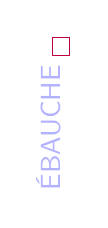
\begin{tikzpicture}
			\node [rotate around={90:(0,0)}] at (0,0) {\draftdate};
		\end{tikzpicture}}
	%position background picture absolutely (w.r.t. upper left page corner) on every page
	\AtBeginShipout{
		\AtBeginShipoutUpperLeft{%
			\put(0.6cm,-26.575cm){\xusebox{PageBGPicture}}}}
\fi

% Glossary style
\renewcommand{\glossarypreamble}{\glsfindwidesttoplevelname[\currentglossary]}
\setabbreviationstyle[acronym]{long-short-sc}
%\setglossarystyle{long}
%\setglossarystyle{long4col}
%\setglossarystyle{mcolalttree}			%alttree -> indent between abbr and text, mcol -> two columns
\loadglsentries{glossary} 				%same as \newacronym[]{mof}{mof}{mean outlier fraction}
\newacronym[]{dom}{dom}{dissolved organic matter}
\newacronym[]{ha}{ha}{humic acid}
\newacronym[]{pet}{pet}{poly(ethylene-terephthalate)}

\newglossaryentry{gamma}
{
	name = {\ensuremath{\gamma}},
	description = {mass concentration},
	sort = {mass c}, 
	type = symbols
}

%\glsdisablehyper 						%no hyperlinks for any gls entry
\renewcommand*{\glsnamefont}[1]{\textsc{\mdseries #1}}   % need to solve the issue with nomeclature entries being \sl\sc like the abbreviations
\renewcommand*{\glstextformat}[1]{\textcolor{black}{#1}} % black hyperlinks!
%\setlength\glsdescwidth{1.5\textwidth}  %does nothing !!

% PAGE CORNERS
\newlength{\brule}	\setlength{\brule}{\topmargin+\headheight+\headsep+\textheight+\footskip}
\tikzset{corner/.pic={code={\draw (0,\headheight)--(0,0)--(\headheight,0);}}}

\AddToShipoutPictureBG{
    \begin{tikzpicture}[remember picture, overlay,color=secondarycolor,]
		\coordinate (O) at ($(current page.north west)$);
        \path ($(O)+(2,-\brule-2.54cm-0.4pt)$) pic {corner};					% bottom-left
        \path ($(O)+(19,-\brule-2.54cm-0.4pt)$) pic[rotate=90] {corner};		% bottom-right
		\path ($(O)+(19,\xrule+\headheight+0.4pt)$) pic[rotate=180] {corner};	% top-right
		\path ($(O)+(2,\xrule+\headheight+0.4pt)$) pic[rotate=270] {corner};	% top-left
    \end{tikzpicture}
}
% APPENDIX
\newleadpage[empty]{Annexes}{%
	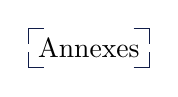
\begin{tikzpicture}
		\node (title) {Annexes};
		\colorlet{casecolor}{titlecolor}%
		\draw[draw=casecolor,line width=0.4pt] ($(title.north west)+(0.2cm,0)$)--(title.north west) -- ++(0,-0.2cm);
		\draw[draw=casecolor,line width=0.4pt] ($(title.south west)+(0,0.2cm)$)--(title.south west) -- ++(0.2cm,0);
		\draw[draw=casecolor,line width=0.4pt] ($(title.north east)+(-0.2cm,0)$)--(title.north east) -- ++(0,-0.2cm);
		\draw[draw=casecolor,line width=0.4pt] ($(title.south east)+(-0.2cm,0)$)--(title.south east) -- ++(0,0.2cm);
	\end{tikzpicture}}

\newleadpage[empty]{Test}{%
	\begin{tikzpicture}[overlay, remember picture]
		\node[outer sep=0,inner sep=0,anchor=north west] at ($(current page.north west)$) (pic)
			{\includegraphics[width=\pagewidth,keepaspectratio=true]{Figures/logos/MPs-on-beach.jpg}};%
		\node[anchor = south west, below = 4pt of pic]
			{\sffamily \textsc{Geographical}, The toxic impact of microplastics in the human body, 3/10/2019};
	\end{tikzpicture}
	Z}

\renewcommand{\parttitlefont}{%
	\fontsize{30pt}{30pt}\titlefamily\scshape\color{titlecolor}}

% ETOOLBOX
\AtBeginEnvironment{tabularx}{\par\addfontfeature{Numbers=Lining}}
\appto\frontmatter{%
	\pagestyle{plainfrontmatter}%
	\aliaspagestyle{chapter}{plainfrontmatter}%
	\chapterstyle{frontmatter}%
	\hypersetup{linkcolor=black}%					% roman numbering, star takes off the numbering
	\microtypesetup{protrusion=false}}

\appto\mainmatter{
	\pagestyle{clean}%
	\aliaspagestyle{chapter}{plainmainmatter}%
	\chapterstyle{main}}

\appto\backmatter{%
	\pagestyle{clean}	%no header, footer is only folios
	\aliaspagestyle{chapter}{plainmainmatter} %pagestyle of the chapterpage
	\chapterstyle{frontmatter}
	\onecolumn}


\renewcommand{\thefootnote}{\roman{footnote}} % Footnotes are latin numbered

% Add a period to the end of an abbreviation unless there's one
% already, then \xspace.
\makeatletter
\DeclareRobustCommand\onedot{\futurelet\@let@token\@onedot}
\def\@onedot{\ifx\@let@token.\else.\null\fi\xspace}
\def\eg{\emph{e.g}\onedot} \def\Eg{\emph{E.g}\onedot}
\def\ie{\emph{i.e}\onedot} \def\Ie{\emph{I.e}\onedot}
\def\cf{\emph{c.f}\onedot} \def\Cf{\emph{C.f}\onedot}
\def\etc{\emph{etc}\onedot} \def\vs{\emph{vs}\onedot}
\def\wrt{w.r.t\onedot} \def\dof{d.o.f\onedot}
\makeatother

% Hyperref for figure, table, appendix, section and equation referencing
\renewcommand{\figurerefname}{Figure}
\newcommand{\fref}[1]{\hyperref[#1]{\figurerefname~\ref*{#1}}}
\newcommand{\frefA}[1]{\hyperref[#1]{\figurerefname~\ref*{#1}\textsc{a}}}
\newcommand{\frefB}[1]{\hyperref[#1]{\figurerefname~\ref*{#1}\textsc{b}}}
\newcommand{\frefC}[1]{\hyperref[#1]{\figurerefname~\ref*{#1}\textsc{c}}}
\newcommand{\frefD}[1]{\hyperref[#1]{\figurerefname~\ref*{#1}\textsc{d}}}
\newcommand{\frefAB}[1]{{\hyperref[#1]{\figurerefname~\ref*{#1}\textsc{a}}} and {\hyperref[#1]{\ref*{#1}\textsc{b}}}}
\newcommand{\frefCD}[1]{{\hyperref[#1]{\figurerefname~\ref*{#1}\textsc{c}}} and {\hyperref[#1]{\ref*{#1}\textsc{d}}}}

\renewcommand{\tablename}{Table}
\newcommand{\tref}[1]{\hyperref[#1]{\tablename~\ref*{#1}}}

\newcommand{\Aname}{Appendix}
\newcommand{\Aref}[1]{\hyperref[#1]{\Aname~\ref*{#1}}}

\newcommand{\Ename}{Equation}
\newcommand{\Eref}[1]{\hyperref[#1]{\Ename~\ref*{#1}}}

\newcommand{\inputpgft}[3][\@empty]{%
	\begingroup
		\renewcommand{\rmfamily}{\liningmainfont}%
		\input{#2}%
		\ifx \@empty#1 \caption{#3}\else \caption[#1]{#3}\fi%
		\vspace{\onelineskip}%
		\begin{tikzpicture}[remember picture, overlay,color=secondarycolor,]
			\coordinate (O) at ($(17,0)$);
			\draw (\headheight,0)--(17cm-\headheight,0);
		\end{tikzpicture}
	\endgroup
}%
\newcommand{\inputpgfb}[3][\@empty]{%
	\begingroup
		\begin{tikzpicture}[remember picture, overlay,color=secondarycolor,]
			\coordinate (O) at ($(17,0)$);
			\draw (\headheight,0)--(17cm-\headheight,0);
		\end{tikzpicture}%
		\vspace{\onelineskip}%
		\renewcommand{\rmfamily}{\liningmainfont}%
		\input{#2}%
		\ifx \@empty#1 \caption{#3}\else \caption[#1]{#3}\fi%
	\endgroup
}%
\newcommand{\inputpd}[3][\@empty]{%
	\begingroup
		\ifx \@empty#1 \caption{#3}\else \caption[#1]{#3}\fi%
		\input{#2}% % par finish the paragrpah so that dotfill starts on new line
  \endgroup
}%
\newcommand{\Chapter}[1]{%
	\chapter{#1}%
	\begin{strip}
		\hypersetup{linkcolor=black}
		\textcolor{insagrey!10}{\noindent\hrule}%
		\vskip 0.5\onelineskip
		\startcontents[sections]
		\printcontents[sections]{}{1}[2]{}	% 1 is startlevel (section=1, chapter=0 )
		\textcolor{insagrey!10}{\noindent\hrule}
		\par\vspace*{4\halfboxsize}\null
		\hypersetup{linkcolor=pink}
	\end{strip}
	\chaptermark{\currentchaptertitle}%
}
\newcommand*\TransitionPic{%
	\clearpage
	\mbox{~}
	\begin{tikzpicture}[overlay, remember picture]
		\node[outer sep=0,inner sep=0,anchor=north west] at ($(current page.north west)$) (pic)
			{\includegraphics[width=\pagewidth,keepaspectratio=true]{Figures/logos/MPs-on-beach.jpg}};%
		\node[anchor = south west, below = 4pt of pic]
			{\sffamily \textsc{Geographical}, The toxic impact of microplastics in the human body, 3/10/2019};
	\end{tikzpicture}
	\clearpage
	\mbox{~}}



\begin{document}
\pagenumbering{Alpha}
%-------Titlepage logo---- from UoM template @alexcasson
\newlength{\logowidth}    \setlength{\logowidth}{40.006mm}
\newlength{\logoheight}   \setlength{\logoheight}{19.454mm}

\newcommand{\MYhref}[3][blue]{\href{#2}{\color{#1}{#3}}}%

\newlength{\logoheightA}\newlength{\logoheightB}\newlength{\logoheightC}
\settoheight{\logoheightA}{\includegraphics[width=\logowidth]{\myhostunilogo}}
\settoheight{\logoheightB}{\includegraphics[width=\logowidth]{\myunilogo}}
\settoheight{\logoheightC}{\includegraphics[width=\logowidth]{\mylablogo}}

\newlength{\vmargin}	\setlength{\vmargin}{\logoheightA+\logoheightB+\logoheightC+\logopad+2cm}
\newgeometry{left = \logowidth+\logopad +1.25cm,right = 20mm,top=\vmargin,bottom = 10mm}

\begin{titlingpage*}
	\AddToShipoutPictureBG*{ % Making sure no corners are shown on titlepage
    \begin{tikzpicture}[remember picture, overlay,color=white,]
		\coordinate (O) at ($(current page.north west)$);
        \path ($(O)+(2,-\brule-2.54cm-0.4pt)$) pic {corner};					% bottom-left
        \path ($(O)+(19,-\brule-2.54cm-0.4pt)$) pic[rotate=90] {corner};		% bottom-right
		\path ($(O)+(19,\xrule+\headheight+0.4pt)$) pic[rotate=180] {corner};	% top-right
		\path ($(O)+(2,\xrule+\headheight+0.4pt)$) pic[rotate=270] {corner};	% top-left
    \end{tikzpicture}}
    \noindent
    \begin{tikzpicture}[overlay, remember picture]
		\node[outer sep=0,inner sep=0,anchor=north west] (A) at ($(current page.north west)+(\logopad,-\logopad)$){%
		\href{www.ctan.org}{\includegraphics[width=\logowidth,keepaspectratio=true]{\myhostunilogo}}%
		};%
		\node[outer sep=0,inner sep=0,anchor=north west,below=0.5cm of A] (B) {%
		\href{www.ctan.org}{\includegraphics[width=\logowidth,keepaspectratio=true]{\myunilogo}}%
		};%
		\node[outer sep=0,inner sep=0,anchor=north west,below=0.5cm of B] (C) {%
		\href{www.ctan.org}{\includegraphics[width=\logowidth,keepaspectratio=true]{\mylablogo}}%
		};%
		\coordinate[below=0.5cm of C] (P);
		\coordinate (L) at ($(P)-(\logowidth/2,0)$);
		\coordinate (center) at ($(L)+(0.5cm+\logowidth,0)$);

		\draw (L)--($(L)+(21cm-2\logopad,0)$);
		\draw 	%vertical line full
			($(current page.north)+(-10.5cm + \logowidth+\logopad+0.5cm,-\logopad)$) -- ($(current page.south)+(-10.5cm + \logowidth+\logopad+0.5cm,\logopad)$);
		\def\side{\logopad/2}
		\fill[fill = white] (center) circle [radius = \side];
		\node at (center) {\HUGE\ding{70}};
	\end{tikzpicture}%
	\linespread{0.7}%
	\sffamily\RaggedRight
	{\hyphenpenalty = 5000 \noindent\Huge\textcolor{insagrey}{\textsc{\documenttype}}\\}%
	\vspace{1\logopad}%
	\linespread{0.7}%
	{\hyphenpenalty = 5000 \scshape\HUGE\color{ecnblue}\thetitle\\}
	%\textbf{{\fontfamily{\family} Assessing the aggregation behaviour of model nanoplastic particles}}
	%{\ag Assessing the aggregation behaviour of model nanoplastic particles}
	%
	\vspace{1\logopad}
	{\HUGE{\textsc{\MYhref[ecnblue]{mailto:\myemail}{\author}}\\}}
	%
	\vspace{1\logopad}
	{\Large\textcolor{ecnblue}{\textit{\myhomeuni}}\\}
	{\Large\textcolor{insagrey}{\textit{\mymastersname}}\\}
	\vspace{4pt}
	\linespread{0.7}
	{\Large\textcolor{ecnblue}{\textit{\myerasmusuni}}\\}
	{\Large\textcolor{insagrey}{\textit{\myerasmusmastersname}}\\}
	%
	\linespread{0.7}
	\vspace{\logopad}
	{\Large\textcolor{insagrey}{\textsc{encadré par}}\\}
	{\huge{\textsc{\MYhref[ecnblue]{mailto:\tutoremail}{\tutor},}}\\}
	{\huge{\textsc{\MYhref[ecnblue]{mailto:\PIemail}{\PI}}\\}}
	%
	\vspace{\logopad}
	{\Large\textcolor{insagrey}{\textsc{référant école}}\\}
	{\huge{\textsc{\MYhref[ecnblue]{mailto:\SchoolSupervisoremail}{\SchoolSupervisor}}\\}}
	%
	\vspace{1\logopad}
	%{\Large\textcolor{insagrey}{\textsc{periode}\\}}
	{\huge\textcolor{insagrey}{\textsc{\timespend}}\\}
\end{titlingpage*}
\restoregeometry

%----------------------------------------------------------------
%   Front Matter
%----------------------------------------------------------------
\frontmatter				% roman pagination
\tableofcontents* 			% starred makes content do not appear in the ToC
\listoffigures
\listoftables
\microtypesetup{protrusion=true}
\hypersetup{linkcolor=titlecolor}

\cleardoublepage
\abstractnum   % Format heading as chapter
\abstractintoc 
\newgeometry{left=4cm, right = 4cm, top=3.125cm, bottom = 20mm}
\onecolumn
\begin{abstract}
\noindent
	\lipsum[1] 
\end{abstract}
\twocolumn
\restoregeometry


\printglossary[type=acronym,title = {Table des abréviations}]
\printglossary[type=symbols,title={Nomenclature}]


%----------------------------------------------------------------
%   Main Matter
%----------------------------------------------------------------
%\TransitionPic
\mainmatter 					% arabic pagination

\Chapter{About the template}
\section{Foreword}
This template must be compiled with the Lua\LaTeX\ engine. The latter supports modern also called smart fonts (which are used in this document) and some nice packages such as \texttt{piton.sty} for including your mind bending vibe coded python scripts. This engine has become over the years the recommended compiler for \TeX. Even though I inted to use this template for projects within Europe, it was made with the \textsf{memoir} class and not the more European-adapted \textsf{koma-script}. Nonetheless, \textsf{memoir} provides many functionalities of which many are used through this document.

\section{The page setup}
As you've now noticed, the body text is separated in two columns. This is done by specifying \texttt{twocolumn} as an option when calling \verb!\documentclass{memoir}!. This layout allows to maximize the usage of paper (both good for printing and scrolling purposes) while in the meantime allowing for high legibility. In my opinion, it is also the best looking layout when one has large figure panels that don't usually fit within the body text width of legible one column documents. However, two columns also means no margin annotations and figures.

\section{The overall structure}
Lines you are reading now are within the main matter \enquote{part} of this document. This is where document divisions are numbered, either by numbers for parts, chapters, sections, etc\dots\ or by letters for the appendix material. All the content before sat in the front matter and is usually unnumbered. The same goes for the backmatter in which indexes and the bibliography go.

\section{A quick word on the babel package}
As you may know, \TeX\ and subsequent \LaTeX\ were engineered by \textsc{us} citizens. Therefore, the engine typesets according to American typographic rules. For the rest of us, we can ensure proper formatting accordingly to our respective region by loading the \verb!babel.sty! package. To do so, make sure your region is given as an option in the document class, say \verb!\documentclass[french]{memoir}! and no package is loaded before \verb!\usepackage[provide=*]{babel}!. As packages are already set accordingly, you should only be changing the region option in the document class.

\section{Looks and customisation}
\subsection{Make it yours!}
This version of the template was compiled with the colors of my engineering school. To do so, the color parameters \texttt{titlecolor} and \texttt{secondarycolor} were set by their \textsc{rgb} code, thanks to the \verb!xcolor.sty! package. Their encoding can be changed at will to match your needs, see lines 5 to 10 in \texttt{common-packages.tex}.

There are two font types used in this document. The bodytext is typed in a classic seriffed font, Palatino Linotype, via its OpenType clone \TeX\ Gyre Pagella. The latter can be changed with the \texttt{\textbackslash setmainfont} command provided by \texttt{fontspec.sty}. Titles, page folios (pagination numbers), float labels and headers are typed in \TeX\ Gyre Adventor. This can be modified by changing the \texttt{\textbackslash setsansfont} command. Maths are also typeset in Palatino, via \verb!\setmathfont{TeX Gyre Pagella Maths}!. The use of \TeX\ Gyre fonts, which are smart font clones of classic font types might require the install of the tex-gyre and tex-gyre-maths packages on the \LaTeX distribution you are using.

When starting a new chapter, one might also want to print its outline under the title, as it was done here. To do so, the writer will call \verb!\Chapter{<title>}! in lieu of the typical \verb!\chapter! command. For better font consistency, looks and optimal resolution, I encourage the reader to make use of the \texttt{pgfplots} package for including their Figures. If so, to make sure numbers are lining and not in oldstyle, one may use the \verb!\inputpgft! and \verb!\inputpgfb! commands, see \fref{fig:fig1} for an examle of their usage.

\subsection{Lettrine}
\lettrine[lines = 3,findent = 4pt, nindent=0pt]{I}{f one would like to include lettrines}, they can do so via the \texttt{lettrine} package which use initials from the \texttt{cfr-initial} package. \texttt{findent} is space between lettrine and first line. \texttt{nindent} is shift of indented lines to that of the first line.

\section{Glossary}
This template comes a with a glossary. To make use of it define entries in the \verb!glossary.tex! file. Items can then be called by \verb!\gls! and friends commands.
The glossary is printed in the front matter, in two tables, one for abbreviations and another for symbols. The \texttt{glossary} package offers lots of customisation for theses tables. With my setup, making the glossary will require installing
\begin{itemize}
	\item the \verb!xindy! package and
	\item the perl software if it is not installed on your computer.
\end{itemize}
If your not interested by a glossary, load the \verb!main.tex! file and get rid of
\begin{itemize}
	\item \verb!\makeglossaries! and
	\item all \verb!\printglossary! commands.
\end{itemize}

\Chapter{RAS}
\section{Some blind text to read}
\begin{figure*}[t]
    \inputpgft[Hello]{Figures/test2.pgf}{%
    This is a caption. \lipsum[2]
    \label{fig:fig1}}
\end{figure*}
\lipsum[1-3]

\begin{itemize}
	\item This is my first bullet point. It's such a pleasure writing. I love my life.
	\item This is my first bullet point. It's such a pleasure writing. WARZAZAT 1994.
\end{itemize}

\begin{table*}
	\caption{\lipsum[2]}
	\begin{tabularx}{\textwidth}{
			>{\RaggedRight\hsize=0.8\hsize\linewidth=\hsize}X
			>{\RaggedRight\hsize=0.8\hsize\linewidth=\hsize}X
			>{\RaggedRight\hsize=0.8\hsize\linewidth=\hsize}X
			>{\RaggedLeft\hsize=1.6\hsize\linewidth=\hsize}X
			}
\toprule
$d$ / nm & medium & $\gls{gamma}_{\gls{pet}}$ / ppm &  \gls{mof} / \% \\
\midrule
\multirow[t]{3}{*}{60} & 1 ppm \gls{ha} & 10 & 6.2 \\
\cmidrule(lr){2-4}
 & \multirow[t]{2}{*}{No \gls{dom}} & 1 & 23.4 \\
 &  & 10 & 3.9 \\
\cmidrule(lr){1-4} \cmidrule(lr){2-4}
\multirow[t]{3}{*}{150} & 1 ppm \gls{ha} & 10 & 0.7 \\
\cmidrule(lr){2-4}
 & \multirow[t]{2}{*}{No \gls{dom}} & 1 & 5.2 \\
 &  & 10 & 0.3 \\ %\arrayrulecolor{secondarycolor}
 \bottomrule
\end{tabularx}

\end{table*}
\section{Second Section}
%
\lipsum[1-5]
\begin{equation}
	\dfrac{r_z(t)}{r_1} = 1 + \dfrac{t}{\tau} + o\left( \dfrac{t}{\tau} \right)
\end{equation}
First citation \cite{calabro-souza_understanding_2026}. \slashfrac{3}{4}. Nice \fref{fig:fig1}.


% APPENDIX
\stopcontents[sections] 		% necessary so that Appendixes do not appear in the last partial ToC.
\Annexes*						% not necessary:  an empty-lead page with "Annexes" written, *for no ToC entry
\appendix						% make chapters alphabetically numbered
\chapter{Numerical methods}
\lipsum[1-3]

%----------------------------------------------------------------
%   Back Matter
%----------------------------------------------------------------
%\TransitionPic
\backmatter
\printbibliography

\end{document}

%\renewcommand{\abstractname}{Acknoledgments}
%\renewcommand{\abstractintoc}{\abstractname}
%\begin{abstract} \input{acknoledgments}\end{abstract}
